\documentclass[11pt]{article}
\usepackage[margin=1in]{geometry}

\usepackage{amsmath}
\usepackage{amssymb}
\usepackage{physics}
\usepackage{graphicx}

\usepackage{tikz}
\usetikzlibrary{shapes.multipart}

\usepackage{subcaption}

\usepackage{hyperref}

\renewcommand{\d}[2][]{\mathrm{d}^{#1}{#2}}



\begin{document}


\section{Introduction}


\begin{itemize}
    \item 1605.01735, \textit{Machine Learning Phases of Matter}, Carrasquilla \& Melko: Used supervised learning with neural-network to classify raw spin configurations into two phases for classical Ising model, square-ice model and gauged Ising model. The trained network for the square-lattice classical Ising model correctly identifies the critical temperature for triangular-lattice classical Ising model without ``information about the Hamiltonian, the lattice structure, or even the general locality of interactions". For the square-ice and gauged Ising models where there is no conventional order parameter, the are able to distinguish between the ground and high-temperature states.
    \item 1606.00318, \textit{Discovering Phase Transitions with Machine Learning}, Lei Wang: Used the unsupervised methods of PCA and clustering to identify phase transitions and order parameters using raw spin configurations in classical Ising model and COP Ising model ($\sum\sigma=0$).
    \item 1609.02552, \textit{Machine Learning Phases of Strongly Correlated Fermions}, Ch'ng et.al.: Used neural-network to identify phases in 3d Hubbard model of fermions on cubical lattice.
    \item 1610.02048, \textit{Learning Phases of Matter by Confusion}, van Nieuwenburg et.al.: Unsupervised methods of PCA and clustering on the entanglement spectrum or Kitaev model clearly identifies different topological phases. Supervised learning with neural-network identifies phases as well, even when omitting a region around the phase-transition point. Their ``confusion scheme" systematically trains on data incorrectly labelled according to a tunable parameter. Asking when the accuracy of the trained network is highest on the entire data set narrows in on the ``correct" value of the parameter and thus the location of the phase transition. This scheme is applied to the classical Ising model in 2d and the random-field Heisenberg chain.
    \item 1703.02435, \textit{Unsupervised learning of phase transitions: from principal component analysis to variational autoencoders}, Wetzel: Used unsupervised methods of PCA and variational autoencoder on 2d classical Ising model and 3d XY model.
    \item 1704.00080, \textit{Discovering Phases, Phase Transitions and Crossovers through Unsupervised Machine Learning: A critical examination}, Hu et.al.: Used PCA and autoencoders to identify phase transitions in square and triangular Ising models, biquadratic-exchange spin-one Ising model (highly degenerate). Blume-Capel model (both first- and second-order transitions) and 2d XY model.
\end{itemize}

Some methods:
\begin{itemize}
    \item PCA: dimensionally reduce data to hyperplane where variance is largest (principal axes).
    \item Autoencoder: ``dimensional reduction" idea applied to neural-networks. Have a hidden layer with very few nodes and train the network to reconstruct data similar to input data based just on that hidden layer (put a bottle-neck in neural network).
\end{itemize}


\section{TDA}
For any discrete data set, persistent homology entails a sequence of simplicial complexes ($\alpha$, Vietoris-Rips, \&c.) of varying granularity in which homological cycles first appear and then disappear. The choice in filtration corresponds to different ways to add edges and faces to the simplicial complex as some parameter is varied. This process produces a collection of persistence data consisting of births and deaths, $\{b_i,d_i\}$, for each of the cycles. Persistence diagrams are a way to visualize these topolgically derived data.

The persistence diagram contains information about the size of features in the data. Since such topological data are robust against small perturbations in the original data set, TDA is a useful tool in statistical analyses of many systems.


(Why persistence image is necessary... robustness against sudden appearence of cycles, small perturbations in persistence data, \&c.) To create the persistence image, begin by transforming the persistence data to $\{(b_i,p_i)\}=\{(b_i,d_i-b_i)\}$. Each point is then smoothed, which allows for perturbations in the topological data to have small effects. Choosing gaussians of fixed width, the full density is
\begin{align}
    \rho(x,y) &= \sum_i w(b_i,p_i)\;\frac{1}{2\pi\sigma^2}\exp\left[-\frac{(x-b_i)^2+(y-p_i)^2}{2\sigma^2}\right]
\end{align}
The weighting function should be chosen so that $w(b_i,0)=0$; this ensures that the sudden appearence of a cycle is accounted for smoothly. For simplicity, we choose $w(b_i,p_i)=p_i$. Because of the lattice structure for these spin models the set of possible $(b_i,p_i)$ pairs is discrete, and we find it convenient to compute $\rho$ as
\begin{align}
    \rho(x,y) &= \sum_{(b,p)}N_{b,p}\times w(b,p)\;\frac{1}{2\pi\sigma^2}\exp\left[-\frac{(x-b)^2+(y-p)^2}{2\sigma^2}\right]
\end{align}
for $N_{b,p}$ the frequency of the $(b,p)$ pair. As for choosing $\sigma$, we have a natural length-scale which is the lattice size. Can compare varying choice of $\sigma$.


The persistence image is then the vector obtained by integrating $\rho$ over a series of ``pixels'' (bins):
\begin{align}
    I_\text{p} &= \iint\limits_\text{p}\rho(x,y)\,\d{x}\d{y}
\end{align}
This process can be done for $H_0,H_1,\ldots$ and the respective vectors adjoined or treated separately. Ultimately, we have now a vector in $\mathbb{R}^n$ ($n$ not too large!) which is a representation of the homological structure of the original data set.

\begin{figure}[h]
    \centering
    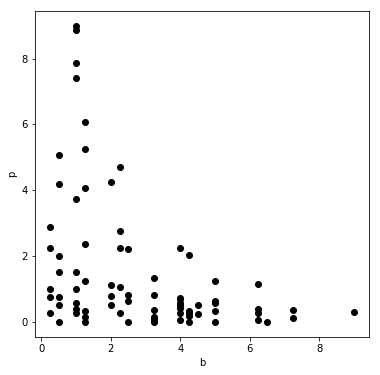
\includegraphics[width=0.3\textwidth]{pd_example}
    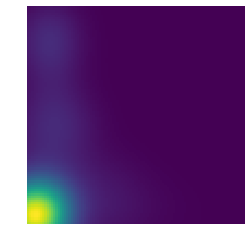
\includegraphics[width=0.3\textwidth]{rho_example}
    
\includegraphics[width=0.3\textwidth]{pi_example}
    \caption{Example PD $\rightarrow\rho\rightarrow$ PI process. Because of the lattice structure many points in the persistence diagram coincide.}
\end{figure}

(The above should be altered slightly for $H_0$ since in this case the persistence data are essentially one-dimensional.)


\newpage
\section{Spin Models}
Here we will apply the techniques of TDA to lattice spin systems. The traditional Ising model is rich in behaviour, despite being simple to describe; in two or more dimensions there is a second-order phase transition from an ordered to random state. While it is relatively easy to distinguish between these states simply by looking at the spin configurations, there exist systems in which the different states are not as readily identified. It has been demonstrated that one can use machine learning to identify phases of matter for such spin systems. We will show that this classification can also be done using persistance images built from the spin configurations, where physical characteristics of the data such as sizes of features play a central role.

We take as data the physical locations of spins which all point in the same direction as the majority of spins after reaching equilibrium with a thermal bath. To generate sample spin configurations, we use Monte Carlo methods, characterized by the following:
\begin{itemize}
    \item $L$: Linear size of periodic lattice. May not correspond to number of spins, e.g.~if spins are not on vertices but on edges.
    \item $\{T_i\}$: Collection of temperatures used.
    \item $N_\text{sim}$: Number of simulations at each temperature.
    \item $K$: Measure of the number of Monte Carlo iterations, being the average number of flips per spin.
\end{itemize}
For each simulation we create a persistence image, which depends on the following choices:
\begin{itemize}
    \item $w(b,p)$: Weighting factor to emphasize longer-lived features. Stability requires $w(b,0)=0$. We choose $w(b,p)=p$ for simplicity.
    \item $\sigma$: Size of gaussians for smoothing process. We have a natural length-scale in our set-up, which is the lattice spacing ($l=1$). Have been using $\sigma=1$, but a comparison for different $\sigma$ would be good to have.
    \item $\{\text{p}_i\}$: Collection of pixels/bins to be integrated over to yield the persistence images. Again, natural scale is set by lattice spacing.
\end{itemize}
After having created these persistence images we have the following methods for identifying phases and critical temperatures:
\begin{itemize}
    \item Logistic regression (supervised learning, identify phase): With a known critical temperature, can train on a subset of the persistence images labelled by their phase. When applied to testing data can quantify accuracy of the regression by comparing to known phase designations.
    \item $k$-means clustering (unsupervised learning, identify phase): Train on a subset of the persistence images, learning appropriate locations for cluster ceneters. When applied to testing data of known temperature can ask what percentage are placed in one cluster or the other, with the critical temperature being where this crosses 50\%. The accuracy at each temperature can also be quantified, since the ``correct'' cluster is known.
    \item PCA (data visualization): Project the high-dimensional persistence images onto the plane for which the variance is largest.
\end{itemize}

The models we choose are increasing non-local. We begin with the classical Ising model, which is exactly solved for $d=2$ and very well-studied for $d=3$. This is the easiest to classify into two phases based on the spontaneous magnetization below the critical temperature. Next is the square-ice (a.k.a.~16 vertex) model, which has no spontaneous magnetization but rather a transition from power-law to exponentially decaying spin-spin correlation functions. Finally, the $\mathbb{Z}_2$-gauged Ising model has a local gauge symmetry which implies no spontaneous magnetization and requires observables to be gauge-invariant in order that they be well-defined. By considering correlation functions aroung loops in the lattice, one finds a phase transition from ``perimeter'' to ``area'' law for $d\geq 3$: there is no phase transition for $d=2$.

\newpage
\section{Classical Ising Model}
As a first example we apply these techniques to the classical Ising model on a cubical lattice. In $d$ dimensions, the Hamiltonian is
\begin{equation}
	H = -\sum_{\langle i,j\rangle}s_is_j \,,
\end{equation}
where $s_i\in\{-1,1\}$ and the sum is over nearest-neighbor vertices of $\mathbb{Z}_L^d$. For all $d\geq2$ there is a second-order phase transition from a disordered phase at high temperatures to an ordered phase at low temperatures. In the thermodynamic limit this critical point is at $T_\text{c}=2/\log{(1+\sqrt{2})}\approx 2.269$ for $d=2$ and $T_\text{c}\approx 4.512$ for $d=3$.

\begin{figure}[h]
	\centering
	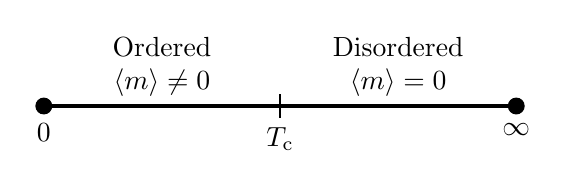
\begin{tikzpicture}[every text node part/.style={align=center}]
		\draw[very thick] (0,0) -- (6,0);
		\draw[fill=black] (0,0) circle (0.1);
		\draw[fill=black] (6,0) circle (0.1);
		\draw[thick] (3,-0.15) -- (3,0.15);
		\node[below] at (0,-0.1) {$0$};
		\node[below] at (6,-0.1) {$\infty$};
		\node[below] at (3,-0.15) {$T_\text{c}$};
		\node[above] at (1.5,0) {Ordered\\ $\ev{m}\neq0$};
		\node[above] at (4.5,0) {Disordered\\ $\ev{m}=0$};
	\end{tikzpicture}
	\caption{Phase diagram for $d\geq2$ classical Ising model with no external field.}
\end{figure}

The presence of spontaneous magnetization as an order parameter makes it easy to distinguishing the two phases by inspection. Examples of spin configurations in the two phases for $d=2$ are shown in figure~\ref{fig:2dIsingExConfigs}.
\begin{figure}[b]
	\centering
	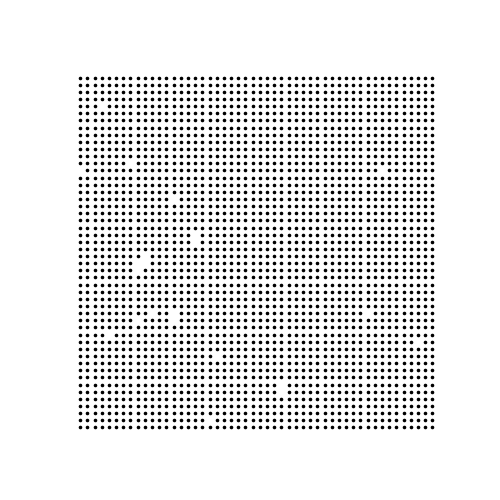
\includegraphics[width=0.35\textwidth]{ising_images/ising_T=150.png}
	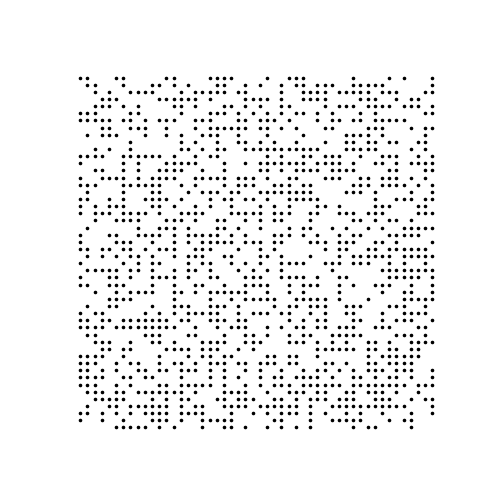
\includegraphics[width=0.35\textwidth]{ising_images/ising_T=inf.png}
	\caption{Example configurations for 2d Ising model at $T=1.5$ (left) and $T=\infty$ (right).}
	\label{fig:2dIsingExConfigs}
\end{figure}

$\vdots$\\

To generate samples weighted by the Boltzmann factor $e^{-\beta H}$, we use the Wolff cluster algorithm on a period lattice with the following parameters:
\begin{equation}
	2d\sim\left\{\begin{aligned}
		L &= 50\\
		\{T_i\} &= \{1.00,1.05,\ldots,3.50\}\\
		N_\text{sim} &= 1400\\
		K &= 20
	\end{aligned}\right. \qquad 3d\sim\left\{\begin{aligned}
		L &= 15\\
		\{T_i\} &= \{3.00,3.05,\ldots,6.00\}\\
		N_\text{sim} &= \\
		K &= 20
	\end{aligned}\right.
\end{equation}
For 2d the persistence diagrams regularly extend out to $b,p\sim25$, and so we choose to create the persistence images using a grid of $25^2$ $1\times1$ pixels. Three such persistence images are shown in figure~\ref{fig:2dExPerIm}.
\begin{figure}[t]
	\centering
%	\includegraphics[width=0.3\textwidth]{ising_images/}
%	\includegraphics[width=0.3\textwidth]{ising_images/}
%	\includegraphics[width=0.3\textwidth]{ising_images/}
	\caption{Example $H_1$ persistence images for 2d Ising model at $T=1.00$ (left), $T=2.30$ (center) and $T=3.50$ (right).}
	\label{fig:2dExPerIm}
\end{figure}



Performing PCA on the persistence images, which live in $\mathbb{R}^{625}$, reveals a striking trend with temperature. The asymmetry in the distribution is due to our choice to always choose the locations of the majority spins (see, e.g., FIG.~5 of [\href{https://arxiv.org/pdf/1703.02435.pdf}{1703.02435}]).

\begin{figure}[h]
	\centering
	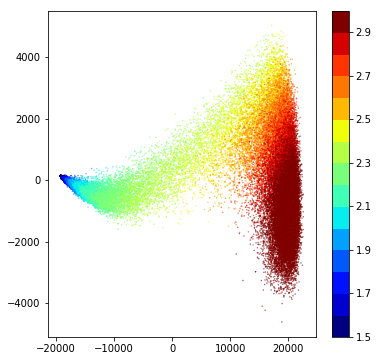
\includegraphics[width=0.4\textwidth]{ising_images/pca_2d_ising}
	\caption{\textbf{IMAGE NOT UP TO DATE} PCA for $H_1$ persistence images of 2d Ising model, colored by temperature.}
	\label{}
\end{figure}

Performing a $k$-means clustering on the 2d $H_1$ persistence images easily separates the data into two clusters. The average cluster label assigned at each temperature is shown in figure~\ref{fig:kMeansAve2dIsing}. The temperature at which half of the samples are placed into each cluster gives an estimate for the critical temperature, $T_\text{c}\approx 2.3246$, with a discrepancy easily attributed to the finite lattice size.

\begin{figure}[h]
	\centering
	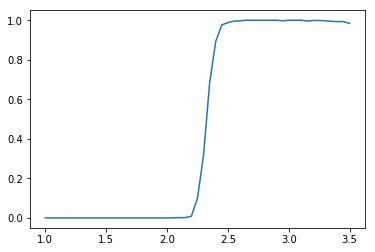
\includegraphics[width=0.4\textwidth]{ising_images/kmeans_avg_2d_ising}
	\caption{$k$-means clustering for $H_1$ persistence images of 2d Ising model.}
	\label{fig:kMeansAve2dIsing}
\end{figure}

$\vdots$

Supervised learning using a logistic regression on the persistence images allows us to identify which topological features are most important in discerning between the two phases. This supervised learning requires the training data to be labelled by phase. To confirm the robustness of this method and account for finite-$L$ effects, we use three labelling schemes characterized by a cut-off temperature, $T_\text{co}\in \{T_\text{c}-0.25,T_\text{c},T_\text{c}+0.25\}$; samples with temperature below $T_\text{co}$ are labelled as being in the ordered phase. The resulting logistic regression coefficients are shown in figure~\ref{fig:LogRegCoef2dIsing}. We see that in all three cases the order parameter has been recovered; the ordered phase is characterized by small, short-lived 1-cycles which we may interpret as small, isolated islands of minority spins.

\begin{figure}[h]
	\centering
	\begin{subfigure}{0.3\textwidth}
		\centering
		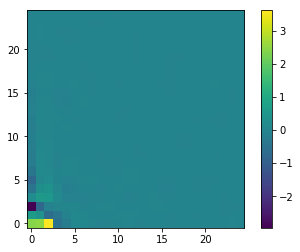
\includegraphics[width=\textwidth]{ising_images/logreg_2d_2019}
		\subcaption{$T_\text{co}=T_\text{c}-0.25$}
	\end{subfigure}
	\begin{subfigure}{0.3\textwidth}
		\centering
		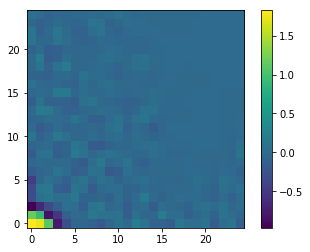
\includegraphics[width=\textwidth]{ising_images/logreg_2d_ising}
		\subcaption{$T_\text{co}=T_\text{c}$}
	\end{subfigure}
	\begin{subfigure}{0.3\textwidth}
		\centering
		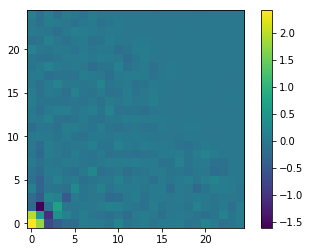
\includegraphics[width=\textwidth]{ising_images/logreg_2d_2519}
		\subcaption{$T_\text{co}=T_\text{c}+0.25$}
	\end{subfigure}
	\caption{Comparison of logistic regression coefficients for three cut-off temperatures for the labelling of the training data.}
	\label{fig:LogRegCoef2dIsing}
\end{figure}

(\textbf{REPEAT ALL FOR 3d})


\subsection{Critical Phenomena}
Near the critical temperature the classical Ising model exhibits scale-invariance and may be described in terms of a scalar CFT. Spin-spin correlation functions for large $r$ are
\begin{equation}
	\ev{s(r)s(0)-m^2} \sim \begin{cases}
		e^{-r/\xi(T)} & T\neq T_\text{c}\\
		r^{-(d-2+\eta)} & T=T_\text{c}
	\end{cases}
\end{equation}
where the correlation length, $\xi(T)$, diverges at the critical temperature. The critical expenent is $\eta=1/4$ in 2d and $\eta\approx0.0363$ in 3d.

Given that the topological data encoded in the persistence diagrams and images is ultimately a result of spins being correlated to give rise to $k$-cycles of various sizes, one could hope to study critical phenomena using TDA.

From the persistence image for $H_k$ one may compute the betti number $b_k$ as a function of scale, by (...). This gives a measure of the frequency of features of a given size in the spin configuration. Fitting $b_1(r)$ to a function of the form
\begin{equation}
	f(r) = c\; e^{-r/\Xi} \,,
\end{equation}	
we find that the correlation length $\Xi$ diverges rapidly around $T_\text{c}$, reaching its largest value at $T=2.xx$.

\bigskip
(PLOT)
\bigskip

Taking a fine-grained view near the critical point where $\Xi$ diverges, we now fit $b_1(r)$ to a function of the form
\begin{equation}
	g(r) = c\; r^{-(d-2+H)}e^{-r/\Xi} \,.
\end{equation}

\bigskip\bigskip
(STILL TO DO: do this fit for $T$ near $T_\text{c}$ and get best estimates for $H$ in 2d and 3d. This will almost surely not give us the critical exponent $\eta$ directly, and likely the mapping from $H\leftrightarrow\eta$ is not so nice/even possible.)


\newpage
\section{Spin-Glass Model}
Perhaps this is interesting? Three phases with two order parameters in 3d (see \href{https://journals.aps.org/prl/pdf/10.1103/PhysRevLett.43.1615}{HERE} for why 2d is not interesting). Also frustration.

\bigskip\bigskip

Take the $\pm J$ Edwards-Anderson Ising model on a cubical lattice, for which the Hamiltonian is
\begin{equation}
	H = -\sum_{\langle i,j\rangle}J_{ij}s_is_j \,,
\end{equation}
where the bonds $J_{ij}$ are assigned values $\pm1$ according to the density function
\begin{equation}
	\mathrm{P}(J_{ij}) = p\,\delta(J_{ij}-1) + (1-p)\,\delta(J_{ij}+1) \,.
\end{equation}
For $p=1$ all $J_{ij}=1$ and this reduces to the classical Ising model.

For $d=3$ there are three phases: ferromagnetic, paramagnetic and spin-glass. The two order-parameters are the magnetization and ():
\begin{equation}
	m \equiv \frac{1}{N}\sum_is_i \,, \qquad\qquad q \equiv 
\end{equation}



\newpage
\section{Square Ice Model}
We consider the square ice model on the cubical lattice $\mathbb{Z}_N^d$ with spins located on edges between adjacent vertices taking values in $\{{-1},1\}$. The Hamiltonian is
\begin{equation}
    H = \sum_v\Big(\sum_{i\ni v}s_i\Big)^2
\end{equation}
where $v\in\mathbb{Z}_N^d$ and by $i\ni v$ we mean those edges connecting to the vertex $v$. We work with a finite lattice of $dN^d$ spins and periodic boundary conditions. At $T=0$ the energy per spin is zero and at $T=\infty$ the energy per spin is two.

This model has a (?-order) phase transition for all $d\geq 2$ as the spin-spin correlation functions go from being power-law at low temperatures to exponentially decaying at high temperatures.

To sample configurations weighted by the Boltzmann factor $e^{-\beta H}$ we use a Monte Carlo algorithm with the following parameters:
\begin{align}
    2d&\sim\left\{\begin{array}{l}
        N = 50\\
        \{T_i\} = \{0.0,0.1,\ldots,4.0\}\\
        N_\text{sim} = 1000(?)\\
        K = 200
    \end{array}\right. & 3d&\sim\left\{\begin{array}{l}
        N = 15\\
        \{T_i\} = \{0.0,0.1,\ldots,4.0\}\\
        N_\text{sim} = 1000(?)\\
        K = 200
    \end{array}\right.
\end{align}
Examples of low- and high-temperature spin configurations are shown in figure~\ref{fig:SquareiceExampleConfigs}. Since the persistence diagrams are very concentrated near the origin, we use $0.5\times0.5$ pixels extending out to $b=5$ and $p=5$ (persistence images are elements of $\mathbb{R}^{100}$).

\begin{figure}[h]
    \centering
    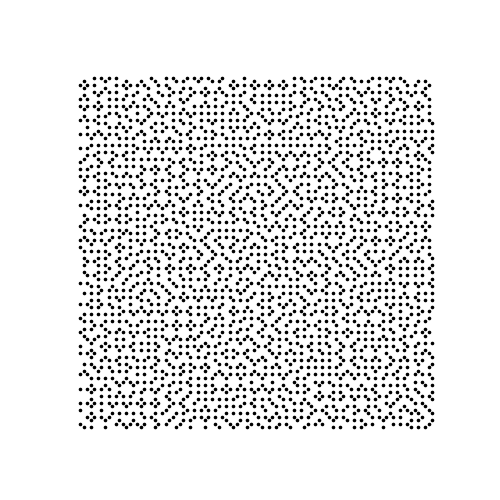
\includegraphics[width=0.28\textwidth]{squareice_images/squareice_T=0.png}
    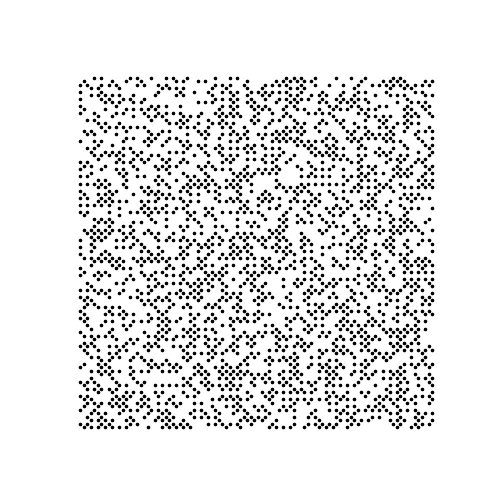
\includegraphics[width=0.28\textwidth]{squareice_images/squareice_T=inf.png}
    \caption{Example configurations for square ice model at $T=0$ (left) and $T=\infty$ (right).}
    \label{fig:SquareiceExampleConfigs}
\end{figure}

\newpage
\subsubsection{$k$-Means}

\begin{figure}[h]
	\centering
	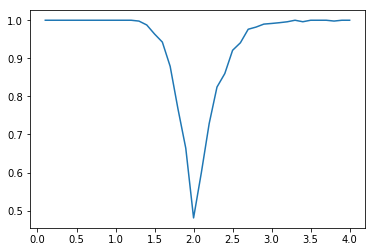
\includegraphics[width=0.3\textwidth]{squareice_images/kmeans_2d_squareice}
	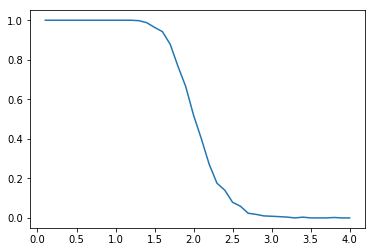
\includegraphics[width=0.3\textwidth]{squareice_images/kmeans_avg_2d_squareice}
	\caption{Left: accuracy on testing data. Right: average classification on testing data. The cross-over point gives an estimate for the critical temperature, $T_\text{c}\approx 2.0166$.}
\end{figure}


\subsubsection{Logistic Regression}
Labelling persistence images using the critical temperature found by $k$-means clustering, can train logistic regression.

\begin{figure}[h]
    \centering
    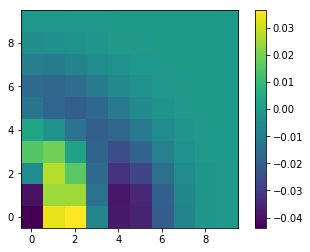
\includegraphics[width=0.3\textwidth]{squareice_images/logreg_2d_squareice}
    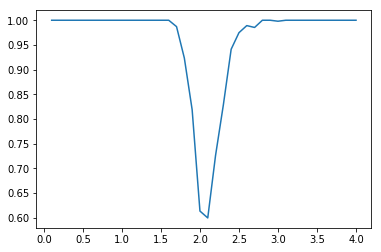
\includegraphics[width=0.3\textwidth]{squareice_images/logreg_acc_2d_squareice}
    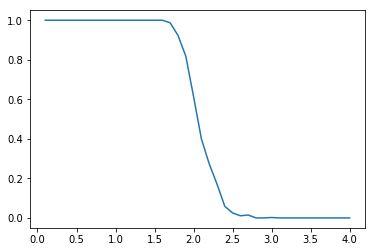
\includegraphics[width=0.3\textwidth]{squareice_images/logreg_avg_2d_squareice}
    \caption{Left: coefficients for logistic regression with $C=0.1$ and $L_2$ penalty. Center: accuracy on testing data. Right: average classification on testing data.}
    \label{fig:SquareiceLogReg}
\end{figure}


\begin{figure}[h]
	\centering
	\begin{subfigure}{0.3\textwidth}
		\centering
		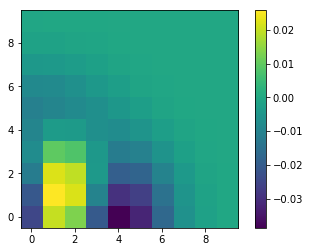
\includegraphics[width=\textwidth]{squareice_images/logreg_2d_181}
		\subcaption{$T_\text{c-o}=1.81$}
	\end{subfigure}
	\begin{subfigure}{0.3\textwidth}
		\centering
		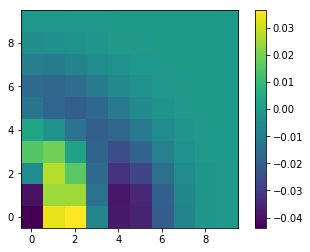
\includegraphics[width=\textwidth]{squareice_images/logreg_2d_squareice}
		\subcaption{$T_\text{c-o}=2.01$}
	\end{subfigure}
	\begin{subfigure}{0.3\textwidth}
		\centering
		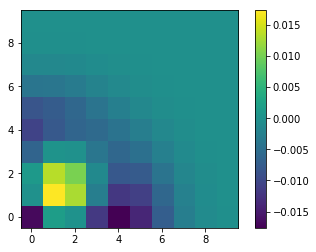
\includegraphics[width=\textwidth]{squareice_images/logreg_2d_221}
		\subcaption{$T_\text{c-o}=2.21$}
	\end{subfigure}
	\caption{Comparison of logistic regression coefficients for three cut-off temperatures for the labelling of the training data.}
\end{figure}


\subsubsection{PCA}
For $d=2$ we have a clear trend in temperature and the projection of the $k$-means clusters reveals the two-cluster structure.
\begin{figure}[h]
    \centering
    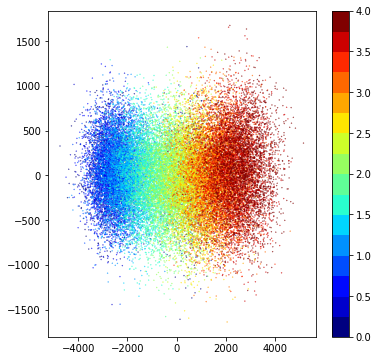
\includegraphics[width=0.25\textwidth]{squareice_images/pca_2d_squareice}
    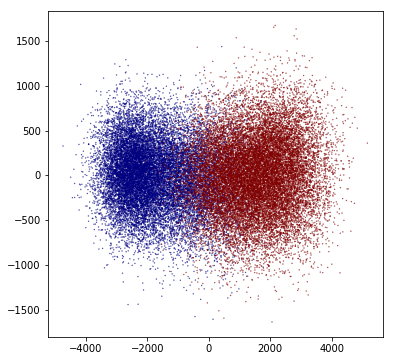
\includegraphics[width=0.26\textwidth]{squareice_images/pca_phase_2d_squareice}
    \caption{Left: PCA colored by temperature. Right: PCA colored by phase, taking $T_\text{c}\approx2.02$.}
    \label{fig:SquareicePCA}
\end{figure}



\newpage
\subsection{$\mathbb{Z}_2$-Gauged Ising Model}
(see [\textit{Gauge fields...}, Balian et.al.])

A variant of the classical Ising model where the global $\mathbb{Z}_2$ symmetry has been promoted to a local (gauge) symmetry is considered as well. The model is defined on the cubical lattice $\mathbb{Z}_N^d$ with spins located on edges between adjacent vertices taking values in $\{{-1},1\}$. The Hamiltonian is
\begin{equation}
    H = - \sum_f\prod_{i\in f}s_i
\end{equation}
where $f$ denote faces, or plaquettes, and by $i\in f$ we mean those four edges consisting of the boundary of $f$. The local $\mathbb{Z}_2$ symmetry corresponds to $H$ being invariant under the flipping of all $2d$ spins on edges connected to any single vertex (this necessarily flips either zero or two spins on each plaquette). We work with a finite lattice of $dN^d$ spins and periodic boundary conditions. At $T=0$ the energy per spin is $\frac{1-d}{2}$ and at $T=\infty$ the energy per spin is zero.

The gauge-invariance guarantees that there is no spontaneous magnetization, and restricting to gauge-invariant observables rules out considering spin-spin correlation functions. An appropriate observable is found by considering a closed path $C$ in the lattice and the expectation value of the product of the spins around this path. In dimensions $d>2$ a phase transition is signalled by a change in such correlation functions: at low temperature one finds a ``perimeter law",
\begin{equation}
    \Big\langle\prod_C s_i\Big\rangle \sim e^{-h(\beta)L} \qquad\qquad h(\beta) = 2e^{-4(d-1)\beta} + \cdots
\end{equation}
while at high temperatures one finds an ``area law",
\begin{equation}
    \Big\langle\prod_C s_i\Big\rangle \sim e^{-f(\beta)A} \qquad\qquad f(\beta) = -\log\operatorname{arctanh}{\beta} + \cdots
\end{equation}
for $L$ the length of the path $C$ and $A$ the minimum number of plaquettes needed to span $C$. The arguments which lead to these expressions do not apply in $d=2$ (see section V.D.~of [\textit{An introduction...}, Kogut]) as the radius of convergence for the validity of the perimeter law is zero. One may also understand the special case of $d=2$ as being a consequence of the equivalence
\begin{equation}
    \big(\text{2d }\mathbb{Z}_2\text{-gauged Ising model}\big) = \big( \text{1d classical Ising model} \big)
\end{equation}
found by comparing the partition functions of the two models after having chosen a convenient gauge. One can, however, still hope to distinguish between high and low temperature spin configurations, as correlation length does change with temperature.

For $d>2$ we can hope to do more: not only identify high and low temperature configuration but also determine the critical temperature at which one shifts from a perimeter to area law.

To sample configurations weighted by the Boltzmann factor $e^{-\beta H}$ we use a Monte Carlo algorithm with the following parameters:
\begin{align}
    2d&\sim\left\{\begin{array}{l}
        N = 50\\
        \{T_i\} = \{0,?\}\\
        N_\text{sim} = 1000(?)\\
        K = 200
    \end{array}\right. & 3d&\sim\left\{\begin{array}{l}
        N = 15\\
        \{T_i\} = \{?\}\\
        N_\text{sim} = 1000(?)\\
        K = 200
    \end{array}\right.
\end{align}
Examples of low- and high-temperature spin configurations are shown in figure~\ref{fig:GaugedExampleConfigs}.

\begin{figure}[h]
    \centering
    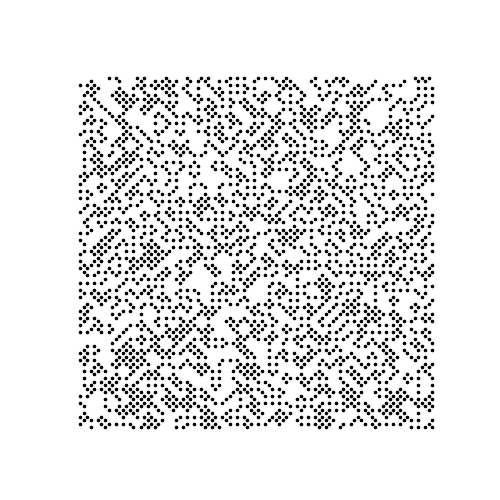
\includegraphics[width=0.3\textwidth]{gauged_images/gauged_T=0.png}
    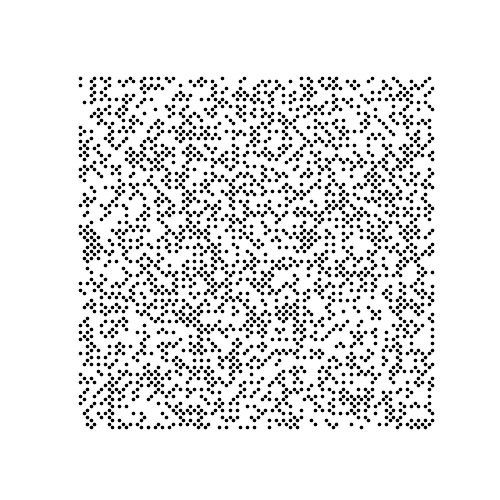
\includegraphics[width=0.3\textwidth]{gauged_images/gauged_T=inf.png}
    \caption{Example configurations for the $\mathbb{Z}_2$-gauged Ising model at $T=0$ (left) and $T=\infty$ (right).}
    \label{fig:GaugedExampleConfigs}
\end{figure}


\subsection{Current Challanges}
K-means and PCA fail, even when using just that subset of the persistence images which are most important for logReg. Why?



\end{document}